\documentclass{article}
\usepackage{tikz}
\usetikzlibrary{arrows.meta}

\begin{document}

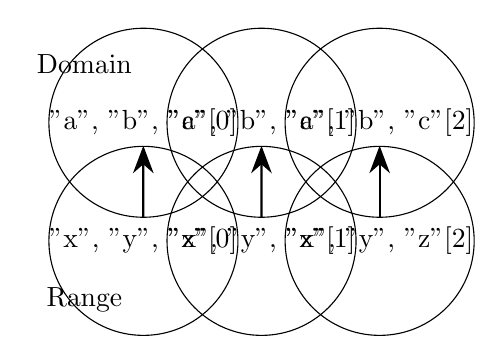
\begin{tikzpicture}[scale=1.5]
    % Define the domain and range sets
    \def\domain{{"a", "b", "c"}}
    \def\range{{"x", "y", "z"}}

    % Draw the domain set
    \node[draw, circle, inner sep=0pt, minimum size=0.2cm] (d1) at (-2, 0) {\domain[0]};
    \node[draw, circle, inner sep=0pt, minimum size=0.2cm] (d2) at (-1, 0) {\domain[1]};
    \node[draw, circle, inner sep=0pt, minimum size=0.2cm] (d3) at (0, 0) {\domain[2]};

    % Draw the range set
    \node[draw, circle, inner sep=0pt, minimum size=0.2cm] (r1) at (-2, -1) {\range[0]};
    \node[draw, circle, inner sep=0pt, minimum size=0.2cm] (r2) at (-1, -1) {\range[1]};
    \node[draw, circle, inner sep=0pt, minimum size=0.2cm] (r3) at (0, -1) {\range[2]};

    % Draw the arrows to show the mapping
    \draw[-{Stealth[scale=1.5]}, thick] (d1) -- (r1);
    \draw[-{Stealth[scale=1.5]}, thick] (d2) -- (r2);
    \draw[-{Stealth[scale=1.5]}, thick] (d3) -- (r3);

    % Add labels for the domain and range
    \node at (-2.5, 0.5) {Domain};
    \node at (-2.5, -1.5) {Range};
\end{tikzpicture}

\end{document}